\chapter{Research Plan}
\label{chap:proposed}
\noindent\textbf{Ph.D. Graduation Estimated Timeline}

\quad\textit{Comprehensive Exam:} Feb 2022

\quad\textit{Proposal Oral:} Mar 2022

\quad\textit{Dissertation Defense:} Feb-Apr 2023\\


\noindent My proposed future work will build on the my work in image classification and V\&L described in the previous chapters by pursuing two key directions:
\begin{itemize}
    \item new algorithms and methods that can improve generalization and robustness of computer vision models, and
    \item analytical and/or theoretical study of the relationship between robustness and domain generalization.
\end{itemize}

\noindent Some of these planned and ongoing projects that are part of this research plan are described below; Table~\ref{tab:research_plan} contains a summary of my contributions.


\section{Empirical Study of Data Modification on Adversarial Robustness}
Generalization and robustness are critical factors that affect the reliability of machine learning models. 
In NLP and vision literature, methods designed for domain generalization report performance on relevant \textit{IID} and \textit{OOD} test sets, but the effect of these methods on adversarial robustness remains unmeasured.
Since methods designed for out-of-domain \textit{(OOD)} generalization are usually a combination of additional training data and new architectures and optimization techniques, we would like to evaluate common categories of methods: training with additional datasets, data augmentation, model debiasing, and data filtering, in comparison with each other.
In this project, we start with identifying five key categories of methods developed for the purpose of increasing out-of-domain generalization or used as baselines.
Our plan is to study the performance of these methods on tasks such as image classification which have standard benchmarks for both OOD generalization as well as adversarial robustness.
Our aim is to understand whether the increase or decrease in OOD generalization by each method over the naive baseline is consistent across tasks.
To further conduct fine-grained analysis, we will also analyze the effect of these methods on in-domain (IID) accuracy on the test set for each task, since in the ideal case improvement in OOD performance should not come at the cost of in-domain accuracy.
Our next aim is to understand the effect of these generalization methods on adversarial robustness.
The results of a synthetic bianry classification task where points lie in a 2-dimensional feature space and separated by concentric circles into class labels.
This setting allows us to visualize the effect of various techniques that alter the training data such as using multiple datasets, automated data augmentation, and algorithmic data filtering, on the training distribution and the resulting performance.
\begin{figure}
    \centering
    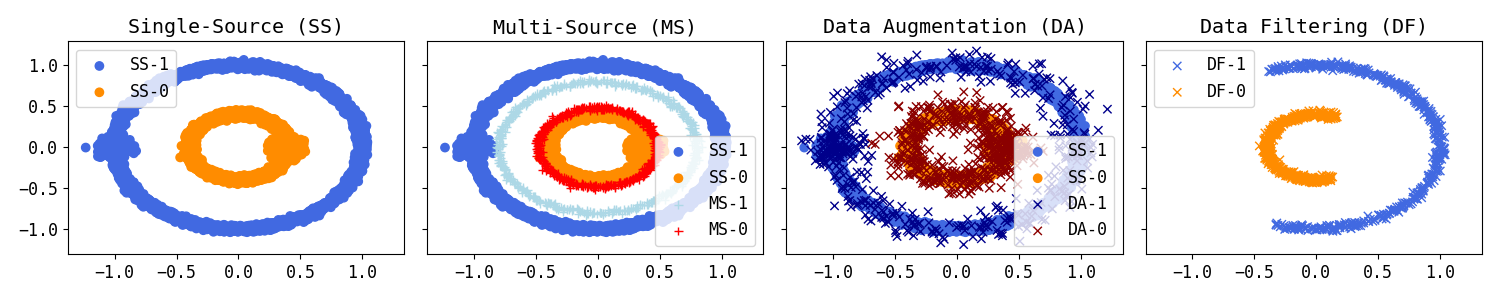
\includegraphics[width=\linewidth]{figures/viz_effect_on_distrib.png}
    \caption{Our toy experimental setting consists of points in $\R^2$ belonging to two classes (0/1).
    This illustration shows the discrepancy between the source dataset (\texttt{SS}) and the out-of-domain dataset (\texttt{OOD}).
    }
    \label{fig:viz_effect_on_distrib}
\end{figure}
% Recent work seeks to understand the relationships between in-domain and out-of-domain performance: for instance,~\citet{miller2021accuracy} empirically show that IID and OOD performance are strongly correlated,~\citet{raghunathan2020understanding,yang2020closer} focus on understanding the tradeoff between robustness and accuracy for adversarially trained models.
% However it is not clear how methods \textit{designed for generalization} affect robustness.
% This is largely because work on domain generalization reports only IID and OOD metrics, and work on robustness reports only IID and robustness metrics.
% This paper seeks to evaluate for the first time, the effect of models designed specifically for generalization on adversarial robustness.
% Our findings can be summarized as follows:
% \begin{itemize}[noitemsep,nosep]
%     \item More data benefits OOD generalization, 
%     \item Data filtering hurts OOD generalization, and
%     \item Data filtering significantly hurts adversarial robustness on all benchmarks.
% \end{itemize}
% % \TG{the sentences that follow can fit well either here or in the conclusion -- decide who to split / tone.}
% These findings and our additional analysis raise new questions for robustness and domain generalization research.
% Significant among these are the importance of both diversity and number of training samples for inductive bias and generalization guarantees, the problems associated with data filtering in terms of robustness, and the importance of a comprehensive set of evaluation metrics that could be adopted for future work.
% In this proposed project, we plan to conduct a comprehensive study of these categories
% on three tasks -- natural language inference (NLI), question answering (QA), and image classification (IC), and evaluate them not only on IID and OOD accuracies, but also on their adversarial robustness (AR).
% We also present results and visualizations on a 2-dimensional synthetic dataset in order to gain grounded insights about the effects of each method on the training distribution.
% Our findings suggest that more data (either via additional datasets or data augmentation) benefits both OOD and AR.
% On the other hand, we find that data filtering (known to improve OOD accuracy on NLI) hurts OOD accuracy on QA and IC, and hurts robustness on all three tasks.

\section{Interpolation as an Analysis Tool for Studying Robustness and Generalization}
We plan to use interpolation between samples from source and target domain in order to understand and characterize model behavior, and obtain a metric for domain shift as a function of this model behavior.

Consider a classification task with label set $\mathcal{Y}$.
For this task, let $\mathcal{X}^{id}$ be the domain from which training images are samples (\textit{id} stands for in-domain).
Let $\mathcal{X}^{od}$ be the domain of images that are out-of-distribution and unseen during training.
In general, $\mathcal{X}^{od}$ can be made of several distinct domains $\mathcal{X}^{od}_1 \dots \mathcal{X}^{od}_{D}$, but we will denote all of them together as  $\mathcal{X}^{od}$ for brevity.
To ground this, we shall use the example of the PACS benchmark where the label set is $\mathcal{Y} = \{ \textrm{`dog' `elephant', `horse', `person', `giraffe', `house', `guitar'}\}$, $\mathcal{X}^{id}$ is a set of photographs, while the $\mathcal{X}^{od}$ is made up of images belong to the same classes, but art/painting, cartoons, and sketches (instead of photographs).

\begin{wrapfigure}{r}{0.5\linewidth}
    \centering 
    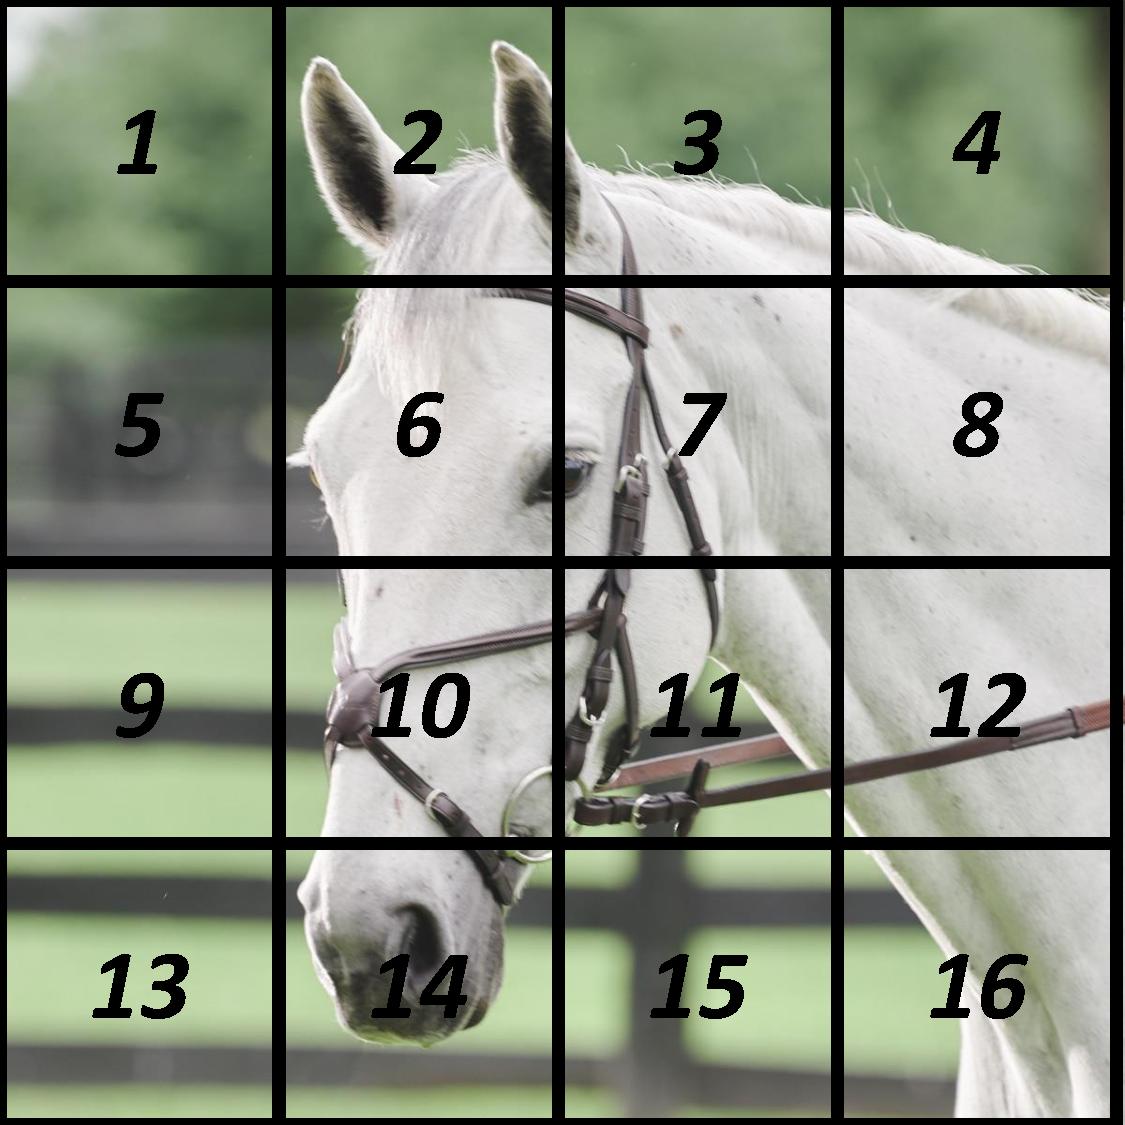
\includegraphics[width=0.6\linewidth]{figures/patch_grid_horse.pdf}
    \caption{Illustration of the division of an image into patches.}
    \label{fig:patch_grid_horse}
\end{wrapfigure}
Now consider a set of classifier models trained on $X_{id}$ until convergence, $\mathcal{F} = \{f_1, \dots, f_K\}$.
We wish to divide each image into a set of non-overlapping patches.
Let this number of patches belong to the set $\mathcal{P}=\{p_1, \dots, p_N\}$.
Given any two images $x_1, x_2$, we interpolate between these two images by randomly selecting one of the $p$ patches from both images and swapping them.
We repeat this process until all patches from image $x_1$ have been replaced by the corresponding patches from $x_2$.
Thus, for $p$ patches, our interpolation method requires $p$ steps of patch-swapping.
At each step $t$, we obtain a resulting \textit{interpolated} image $x_{in}^t (p)$ and for each model $f$, we can obtain class-predictions $y_{in}^t (f, p)$ for these interpolated images.
This intuitive process is explained mathematically in Algorithm~\ref{algo:patchwise_interpolation}.

Thus for each pair of samples $x_1$, $x_2$ we get a sequence of interpolated images and their predictions $X_{x_1, x_2}(p)$ and $Y_{x_1, x_2}(f, p)$ respectively.
From $Y$, we can compute the number of transitions between subsequent predictions -- this measures how frequently the predictions fluctuate from one class label to another during the process of interpolation.
This quantity, $z$, gives us a measure of how sensitive the model $f$ is to interpolations using $p$ patches.
(Note: larger $p$ implies smaller patch size).
Thus we name this quantity \textit{``interpolation sensitivity"} and compute it as:
\begin{equation}
    z_{x_1, x_2} (f, p) = \frac{1}{p}\sum_{i=1}^{p}\mathbbm{1}\Big( Y_{x_1, x_2}(f, p)[i] == Y_{x_1, x_2}(f, p)[i-1]\Big)
\end{equation}

\begin{algorithm}
    \caption{PATCHWISE INTERPOLATION for images}
    \begin{algorithmic}[0]
        \State \textbf{Input:} images $x_1$, $x_2$, model $f$, number of patches $p$
        \State \textbf{Output:} interpolated image sequence $X_{x_1, x_2}(p)$ and output sequence $Y_{x_1, x_2}(f, p)$
    \end{algorithmic}
    \begin{algorithmic}[1]
        \State \textbf{Initialize:} $M = \underline{\mathbf{0}}^{H\times W}$ \algorithmiccomment{\textit{initialize mask as a matrix of all zeros}}
        \ForEach{$t \in \{1\dots p\}$}%
            \State $q \widesim[3]{w/o~repl.} \{1, \dots, p\}$ \algorithmiccomment{\textit{sample patch index without replacement}}
            \State $M[q] \gets 1$ \algorithmiccomment{\textit{set patch $q$ elements to 1}}
            \State $x_{in}^t (p) \gets x_1\odot (1-M) + x_2\odot M$ \algorithmiccomment{\textit{interpolate}}
            \State $y_{in}^t (f, p) \gets f(x_{in}^t (p) $ \algorithmiccomment{\textit{get predicted class}}
        \EndForEach
        \State $X_{x_1, x_2} (p) \gets [x_{in}^1(p) \dots x_{in}^p(p)]^T$
        \State $Y_{x_1, x_2} (f, p) \gets [y_{in}^1(f,p) \dots y_{in}^p(f,p)]^T$
        \State\Return $\theta$
\end{algorithmic}
\label{algo:patchwise_interpolation}
\end{algorithm}



Given this formula for computing pairwise interpolation sensitivity, we can also compute a dataset-level statistic, depending on the domain of $x_1$ and $x_2$.
\begin{align}
    Z^{id-id} (f, p) &= \underset{x_1, x_2 \in \mathcal{X}^{id}}{\E} z_{x_1, x_2}(f, p) \\
    Z^{od-od} (f, p) &= \underset{x_1, x_2 \in \mathcal{X}^{od}}{\E} z_{x_1, x_2}(f, p) \\
    Z^{id-od} (f, p) &= \underset{\substack{x_1 \in \mathcal{X}^{id},\\ x_2\in\mathcal{X}^{od}}}{\E} \frac{1}{2}(z_{x_1, x_2}(f, p) + z_{x_2, x_1}(f, p))
    \label{eq:expected_sensitivity}
\end{align}

Armed with this measure of sensitivity, we can now analyse the correlation between out-of-domain accuracy and interpolation sensitivity.
% Let $\mathfrak{Z}$ denote the $|\mathcal{F}|\times|\mathcal{P}|$ matrix where each elemnt $\mathfrak{Z}[i, j]$ represents the sensitivity of model $f_i$ when interpolating with $p_j$ patches.
Let $\mathbb{A}$ be a $K\times 1$ vector of OOD accuracies of each model.
Then we can compute the Pearson correlation of OOD accuracies with sensitivity values at all values of $p$, as:
\begin{align}
    \rho(p)^{id-id} &= corr(\mathbb{A}, [Z^{id-id}(f_1, p), \dots, Z^{id-id}(f_K, p)])\\
    \rho(p)^{id-id} &= corr(\mathbb{A}, [Z^{od-od}(f_1, p), \dots, Z^{od-od}(f_K, p)])\\
    \rho(p)^{id-id} &= corr(\mathbb{A}, [Z^{id-od}(f_1, p), \dots, Z^{id-od}(f_K, p)])
    \label{eq:correlation}
\end{align}

We plan to develop the above and other analytical measures to understand model behavior and connections with adversarial robustness, corruption robustness, and domain shift.
Our hypothesis is that sensitivity values obtained from patchwise interpolations as defined in Algorithm~\ref{algo:patchwise_interpolation} are indicative of model robustness.
While this study will be largely analytical in nature, theoretical connections between domain shift and robustness may emerge, which would be useful for future research on generalization.


\section{Evaluating Robustness of V\&L Systems}
I am leading a project which aims to analyze the relative contributions of visual and textual inputs in multi-modal tasks by analyzing existing models for captioning, question-answering, and reasoning, through the analytical lens of image generation.
The joint study of text-to-image (T2I) and downstream V\&L tasks can enable us to reason both about the quality of existing image synthesis approaches as well as models trained for tasks such as visual question answering, image captioning, retrieval, etc.
I am currently working on preliminary experiments for this project.

In Summer 2022, I will collaborate with researchers at Microsoft Research -- the aim of this project is closely aligned with my thesis topic of studying robust visual understanding.
We are currently in the brainstorming stage for this project.
% I will investigate how sensitive models are to very small perturbations of object locations, and what are the failure modes of these models when it comes to such ``spatial robustness''.

Table~\ref{tab:research_plan} provides a summary of my publications during my Ph.D. as well as a timeline for planned projects.

% \paragraph{Summary of Contributions}


\begin{table}
    \centering
    % \small
    \resizebox{\linewidth}{!}{
    \begin{tabular}{@{}p{0.48\linewidth}clcl@{}}
        \toprule
        \textbf{Short Title} & \textbf{Lead} & \textbf{Venue} & \textbf{Domain} & \textbf{Task}\\
        \midrule
        Visual Planning~\citep{gokhale2019blocksworld}      & $\checkmark$  & $^W$CVPR-19   & V     & Planning \\
         \textbf{VQA-LOL}~\citep{gokhale2020vqa}            & $\checkmark$  & ECCV-20       & V{+}L & VQA\\
        Video2Commonsense~\citep{fang2020video2commonsense} & $\checkmark$  & EMNLP-20      & V{+}L & Captioning, VQA\\
        \textbf{Mutant}~\citep{gokhale2020mutant}           & $\checkmark$  & EMNLP-20      & V{+}L & VQA\\
        \textbf{AGAT}~\citep{gokhale2020attribute}          & $\checkmark$  & AAAI-21       & V     & Img. Cls. \\
        TTL-RC~\citep{banerjee-etal-2021-self}              &               & NAACL-21      & L     & QA \\
        Halluci-Net~\citep{kulkarni2020halluci}             &               & $^W$CVPR-21   & V     & Image Synthesis \\
        \textbf{WeaQA}~\citep{banerjee2021weaqa}            &               & ACL-21 Findings   & V{+}L & VQA \\ 
        \textbf{SpatialVQA}~\citep{banerjee2021weakly}      &               & ICCV-21       & V{+}L & VQA \\
        \midrule 
        \textbf{SDRO}~\citep{gokhale2021semantically}       & $\checkmark$  & (R) ACL-22    & V{+}L & V\&L Inference \\
        PHL Triplet NLI~\citep{varshney2021unsupervised}&              & (R) ACL-22    & L     & NLI \\
        Poly-DPR~\citep{luo2022improving}                   &               & (R) AAAI-22   & L     & Retrieval \\
        \textbf{ALT}                                        & $\checkmark$  & (R) CVPR-22   & V     & Img. Cls. \\
        \midrule 
        \textbf{Effect of Dataset Modification}~\citep{}    & $\checkmark$  & (R) ACL-22    & V, L  & evaluation \\
        \textbf{Robustness Study via Interpolation}         & $\checkmark$  & (P) NeurIPS-22 & V{+}L & evaluation \\
        \textbf{Unsupervised Spatial VQA}                   & $\checkmark$  & (P) NeurIPS-22 & V{+}L & VQA \\      
        \textbf{Joint Evaluation T2I and V\&L}              & $\checkmark$  & (P) EMNLP-22  & V{+}L & evaluation \\
        \textbf{V\&L Pre-Trained Model Robustness} (with MSR, Summer 2022) & $\checkmark$ & 2023 & V{+}L \\
        \bottomrule
    \end{tabular}
    }
    \caption{
    Chronological publications and future research plan.
    Abbreviations: \textit{$^W$: Workshop proceedings, $\checkmark$: main author, (R): under review, (P): planned submission, V: vision, L: language, \textbf{bold}: described in this proposal
    }
    }
    \label{tab:research_plan}
\end{table}
